%%%%%%%%%%%%%%%%%%%%%%%%%%%%%%%%%%%%%%%%%
% a0poster Portrait Poster
% LaTeX Template
% Version 1.0 (22/06/13)
%
% The a0poster class was created by:
% Gerlinde Kettl and Matthias Weiser (tex@kettl.de)
% 
% This template has been downloaded from:
% http://www.LaTeXTemplates.com
%
% License:
% CC BY-NC-SA 3.0 (http://creativecommons.org/licenses/by-nc-sa/3.0/)
%
%%%%%%%%%%%%%%%%%%%%%%%%%%%%%%%%%%%%%%%%%

%TODO puede ir: trabajo pendiente, explicación de variables si falta, más texto
%TODO cambiar las 2 columnas de itv vs tiempo
%TODO mover logo departamento

%----------------------------------------------------------------------------------------
%	PACKAGES AND OTHER DOCUMENT CONFIGURATIONS
%----------------------------------------------------------------------------------------

\documentclass[a0,portrait]{a0poster}

\usepackage{multicol} % This is so we can have multiple columns of text side-by-side
\columnsep=100pt % This is the amount of white space between the columns in the poster
\columnseprule=3pt % This is the thickness of the black line between the columns in the poster

\usepackage[svgnames]{xcolor} % Specify colors by their 'svgnames', for a full list of all colors available see here: http://www.latextemplates.com/svgnames-colors

\usepackage{times} % Use the times font
%\usepackage{palatino} % Uncomment to use the Palatino font

\usepackage{graphicx} % Required for including images
\graphicspath{{figures/}} % Location of the graphics files
\usepackage{booktabs} % Top and bottom rules for table
\usepackage[font=small,labelfont=bf]{caption} % Required for specifying captions to tables and figures
\usepackage{amsfonts, amsmath, amsthm, amssymb} % For math fonts, symbols and environments
\usepackage{wrapfig} % Allows wrapping text around tables and figures

\usepackage[utf8x]{inputenc}			%acentos, etc
\usepackage[spanish,activeacute]{babel}	%titulos en castellano
\usepackage[version=3]{mhchem}			%química
\usepackage{siunitx}					%unidades

%esto es para que no ponga números en las referencias
\makeatletter
\renewcommand\@biblabel[1]{}
\renewenvironment{thebibliography}[1]
     {\section*{\refname}%
      \@mkboth{\MakeUppercase\refname}{\MakeUppercase\refname}%
      \list{}%
           {\leftmargin0pt
            \@openbib@code
            \usecounter{enumiv}}%
      \sloppy
      \clubpenalty4000
      \@clubpenalty \clubpenalty
      \widowpenalty4000%
      \sfcode`\.\@m}
     {\def\@noitemerr
       {\@latex@warning{Empty `thebibliography' environment}}%
      \endlist}
\makeatother


\begin{document}

\newcommand{\h}{\ce{H^+}}
\newcommand{\oh}{\ce{OH^-}}
\newcommand{\na}{\ce{Na^+}}
\newcommand{\cl}{\ce{Cl^-}}
\newcommand{\kvm}{$\si{\kilo\volt\per\metre}$}
\newcommand{\usec}{$\si{\micro\second}$}

%----------------------------------------------------------------------------------------
%	POSTER HEADER 
%----------------------------------------------------------------------------------------

% The header is divided into two boxes:
% The first is 75% wide and houses the title, subtitle, names, university/organization and contact information
% The second is 25% wide and houses a logo for your university/organization or a photo of you
% The widths of these boxes can be easily edited to accommodate your content as you see fit

\begin{minipage}[b]{0.75\linewidth}
\veryHuge \color{NavyBlue} \textbf{Modelado de Electroporación Celular} \color{Black}\\ % Title
%\Huge\textit{An Exploration of Complexity}\\[2cm] % Subtitle PUEDE IR UN SUBTITULO
%\huge \textbf{John Smith \& James Smith}\\[0.5cm] % Author(s)
%\huge University and Department Name\\[0.4cm] % University/organization
%\Large \texttt{john@LaTeXTemplates.com} --- 1 (000) 111 1111\\

\huge \textbf{Mauricio Alfonso} - LSC, FCEyN\\[0.5cm]
\huge \textbf{Alejandro Soba} - CSC-CONICET\\[0.5cm]
\huge \textbf{Guillermo Marshall} - INFIP, CONICET\\[0.5cm]

\end{minipage}
%
\begin{minipage}[b]{0.25\linewidth}

\includegraphics[width=20cm]{logodc.jpg}\\
\end{minipage}

\vspace{1cm} % A bit of extra whitespace between the header and poster content

%----------------------------------------------------------------------------------------

\begin{multicols}{2} % This is how many columns your poster will be broken into, a portrait poster is generally split into 2 columns

\color{Navy} % Navy color for the abstract

%\begin{abstract}
%\large
\begin{center}Introducción\end{center}
La electroporación reversible es un método consistente en la aplicación de pulsos eléctricos de alta intensidad a una célula con el objetivo de permeabilizar su membrana creando poros, y así permitir el ingreso de drogas o moléculas de ADN a su interior. Esto permite tratar tumores con menores cantidades de drogas, reduciendo los efectos secundarios.\\

En este trabajo se simula una célula esférica a la que se le aplica un pulso eléctrico de 20\si{\milli\second} de duración a través de dos electrodos, y se estudia el ingreso al interior de la célula de 4 especies iónicas: el ión hidrógeno (\h), el hidróxido (\oh), el catión sodio (\na) y el cloruro (\cl). Para eso se tiene en cuenta el campo eléctrico producido por los electrodos, la generación y evolución de poros en la membrana celular producto de la diferencia de potencial entre el interior y exterior de la célula , y la migración de las especies mencionadas, producto de la diferencia de potencial.\\

Las simulaciones se realizaron con el método de elementos finitos sobre mallas bidimensionales que representan el dominio sobre un sistema de coordenadas cilíndricas usando elementos cuadrilaterales.

%\end{abstract}

%\color{SaddleBrown} % SaddleBrown color for the introduction

%\section*{Introduction}
%
%Aliquam non lacus dolor, \textit{a aliquam quam} \cite{Smith:2012qr}. Cum sociis natoque penatibus et magnis dis parturient montes, nascetur ridiculus mus. Nulla in nibh mauris. Donec vel ligula nisi, a lacinia arcu. Sed mi dui, malesuada vel consectetur et, egestas porta nisi. Sed eleifend pharetra dolor, et dapibus est vulputate eu. \textbf{Integer faucibus elementum felis vitae fringilla.} In hac habitasse platea dictumst. Duis tristique rutrum nisl, nec vulputate elit porta ut. Donec sodales sollicitudin turpis sed convallis. Etiam mauris ligula, blandit adipiscing condimentum eu, dapibus pellentesque risus.
%
%\textit{Aliquam auctor}, metus id ultrices porta, risus enim cursus sapien, quis iaculis sapien tortor sed odio. Mauris ante orci, euismod vitae tincidunt eu, porta ut neque. Aenean sapien est, viverra vel lacinia nec, venenatis eu nulla. Maecenas ut nunc nibh, et tempus libero. Aenean vitae risus ante. Pellentesque condimentum dui. Etiam sagittis purus non tellus tempor volutpat. Donec et dui non massa tristique adipiscing.

\color{DarkSlateGray} % DarkSlateGray color for the rest of the content

\section*{Teoría}

%\subsection*{Potencial Eléctrico}
Potencial eléctrico:
			\begin{equation}
				\sigma_{e} \nabla^2 \phi = 0
			\end{equation}

%			Con $\phi$ el potencial eléctrico y $\sigma_{e}$ la conductividad del material.
%			Condiciones de borde de Dirichlet en los electrodos y Neumann en los otros bordes.\\
			
%			El potencial transmembrana (ITV) debería aproximarse a:
%			\begin{center}
%				$V^{\theta} = 1.5 E cos (\theta)$
%			\end{center}

			Se asume que la membrana se carga como un capacitor en paralelo con una resistencia:
			\begin{equation}
				V_m = V_p (1 - e^{-t/\tau}),
%			\end{equation}
%			\begin{equation}
				\textrm{ con } \tau = \alpha C_m \left( \frac{1}{\sigma_i} + \frac{1}{2 \sigma_o} \right)
			\end{equation}\\
			
%			Con $\alpha$ el radio, $C_m$ la capacitancia de la membrana y $\sigma_i$ y $\sigma_o$ las
%			conductividades interna y externa.

	Densidad de poros:
	\begin{equation}
		\frac{\partial N}{\partial t} = \alpha_c e^{(V_m/V_{ep})^2} 
			\left( 1 - \frac{N}{N_0 e^{q \left(V_m/V_{ep} \right) ^2}} \right)
	\end{equation}
	La densidad depende del ITV en cada región de la célula 
	(no es constante en toda la superficie).\\
%	\newline 
	%			$N$ es la densidad de poros, $V_m$ es el ITV, $\alpha_c$ es el coeficiente de creación de poros, 
	%			$V_{ep}$ es el voltaje característico de electroporación, 
	%			$N_0$ es la densidad de poros en equilibrio (cuando $V_m = 0$) y 
	%			$q$ es una constante igual a $(r_m / r*)^2$, donde $r_m$ es el radio de mínima energía 
	%			para $V_m = 0$ y $r*$ es el radio mínimo de los poros.\\

%	$N$ es la densidad de poros, $V_m$ es el ITV, 
%	$\alpha_c$, $V_{ep}$, $N_0$ y $q$ constantes.

	Radio de los poros:
	\begin{equation}
		\frac{\partial r}{\partial t} = \frac{D}{kT} \left( \frac{V_m^2 F_{max}}
			{1+r_h / (r+r_a)} + \frac{4 \beta}{r} \left(\frac{r_*}{r}\right)^4 
			- 2 \pi \gamma + 2 \pi \sigma_{\textrm{\tiny eff}} r\right),			
		\textrm{ con }\sigma_{\textrm{\tiny eff}} = 2 \sigma^\prime - 
			\frac{2 \sigma^\prime - \sigma_0}{(1 - A_p / A)^2}
	\end{equation}
	
	

	%			\begin{center}
	%				$ \textrm{con } \sigma_{\textrm{\tiny eff}} = 2 \sigma^\prime - 
	%					\frac{2 \sigma^\prime - \sigma_0}{(1 - A_p / A)^2}	$
	%			\end{center}

	Se aplica a cada poro por separado.\\


	Transporte de especies: ecuación de Nernst-Planck
	\begin{equation}
		\frac{\partial C_i}{\partial t} = \nabla \cdot \left( D_i \nabla C_i + D_i z_i 
			\frac{F}{R T} C_i \nabla \phi \right)
	\end{equation}	\\			
%	donde $C_i$, $D_i$ y $z_i$ son la concentración, la difusión y la valencia de la 
%		especie $i$, para $i$ alguna de las especies mencionadas (\h, \oh, \na, \cl).
%	\newline \newline		
%	$F$ y $R$ son las constantes de Faraday y de los gases y $T$ la temperatura.

	La conductividad de la membrana se recalcula según el área ocupada por los poros:
	\begin{equation}
		\sigma_{e} = \sigma_m (1 - p) + \sigma_p p
	\end{equation}\\
%	donde $p$ es la proporción ocupada por poros de una zona esférica de la membrana. 
%	$\sigma_m$ y $\sigma_p$ son las conductividades de la membrana sin poros y del líquido 
%	que llena el poro
%	\newline \newline
	Lo mismo se hace con la difusión:
	\begin{equation}
		D_{i, e} = D_i (1 - p) + D_p
	\end{equation}

%	D_m$ y $D_p$ son las conductividades de la membrana sin poros y del líquido 
%	que llena el poro

\section*{Implementación}
\begin{multicols}{2}
	\begin{itemize}
		\item Métodos de elementos finitos para potencial eléctrico (ecuación de Poisson) y transporte de especies
		\item Diferencias finitas para generación y evolución de poros
		\item Implementado en \texttt{C++}
		\item Malla con coordenadas cilíndricas (2D)
		\item Elementos cuadrilaterales
%		\item Librería Eigen para resolver sistemas de ecuaciones
		\item Descomposiciones Cholesky (para Poisson) y Bi-gradientes conjugados estabilizados (para transporte)
		\item OpenMP para acelerar llenado de matrices (Poisson) y resolución en transporte
	\end{itemize}

		\columnbreak
		\begin{center}
			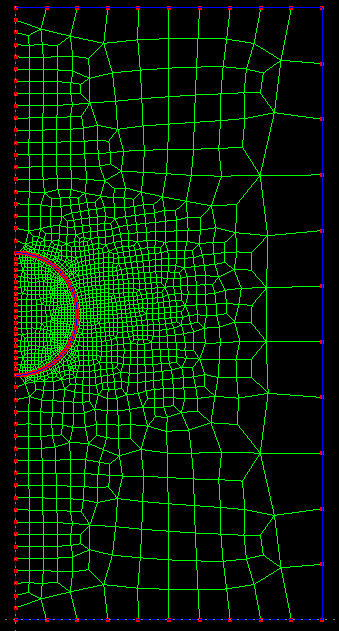
\includegraphics[keepaspectratio, height = 0.18\textheight]{grande} 
			\captionof{figure}{\color{Green}Ejemplo de malla con coordenadas cilíndricas}
		\end{center}

\end{multicols}

\section*{Resultados}

\subsection*{Voltaje Transmembrana (ITV)}
ITV en función del tiempo para diferentes ángulos:

	\begin{multicols}{2}
		\begin{center}\vspace{1cm}
			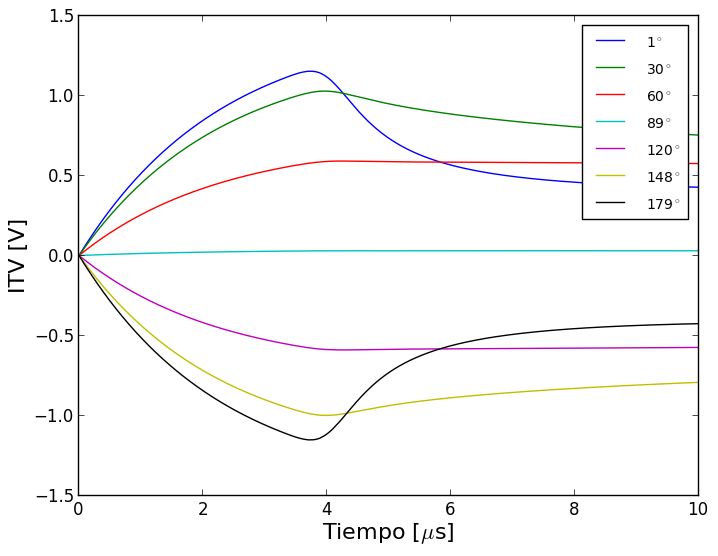
\includegraphics[width=1\linewidth]{itv-time-lin-25-64-40KVm}
			\captionof{figure}{\color{Green}Para $\alpha$ = 25\si{\micro\metre} y 40\kvm}
		\end{center}\vspace{1cm}
	\columnbreak
		\begin{center}\vspace{1cm}
			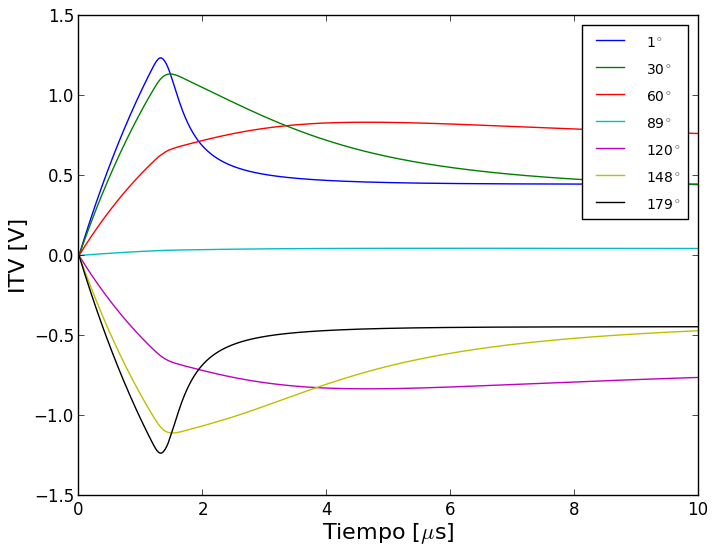
\includegraphics[width=1\linewidth]{itv-time-lin-25-64-80KVm}
			\captionof{figure}{\color{Green}Para $\alpha$ = 25\si{\micro\metre} y 80\kvm}
		\end{center}\vspace{1cm}
	\end{multicols}

\begin{itemize}
	\item En una primera etapa la tensión sube al iniciarse el pulso. Esto no se da de manera inmediata debido a que la membrana se carga como un capacitor. El ITV crece de manera más rápida en las regiones celulares cercanas a los polos, mientras que en las regiones cercanas al ecuador casi no deja de ser cero.
	\item Al alcanzar un pico de tensión, el ITV comienza a disminuir. Esto se debe a que los valores altos de tensión alcanzados crearon poros que aumentan significativamente la conductividad de la membrana, reduciendo su caída de tensión. Este proceso se da de manera más precipitada en las regiones cercanas a los polos, y más lentamente en las regiones cercanas al ecuador. 
\end{itemize}

\begin{multicols}{2}
	ITV en función del ángulo para diferentes instantes
	\begin{center}\vspace{1cm}
	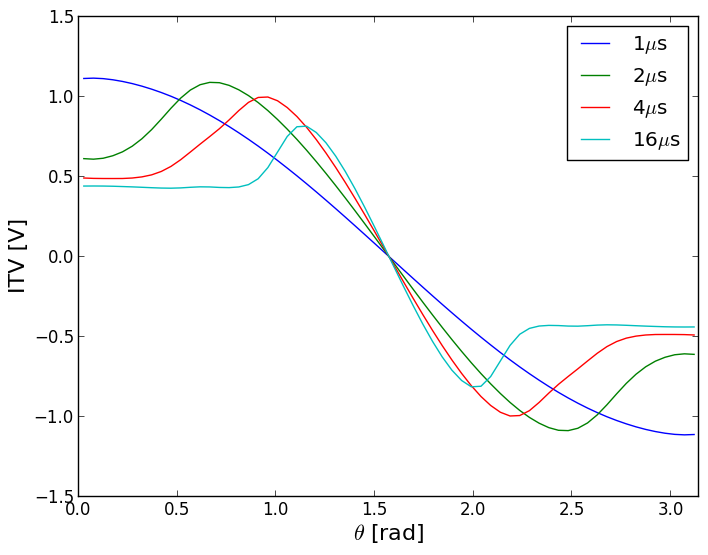
\includegraphics[width=1\linewidth]{itv-tita-50-64-80KVm}
	\captionof{figure}{\color{Green} ITV para $\alpha$ = 50\si{\micro\metre} y 80\kvm}
	\end{center}\vspace{1cm}
	
\columnbreak
	Para que se dé este proceso el campo eléctrico debe alcanzar un umbral mínimo. En los que el potencial necesario fue alcanzado, un incremento en el campo eléctrico aplicado parece prácticamente no influir en los valores de ITV alcanzados, pero sí en la velocidad en la que se produce el proceso descrito. El potencial transmembrana alcanzado casi no varía, influyendo el potencial aplicado solo en la velocidad en la que se producen las variaciones de ITV.\\
\end{multicols}


\subsection*{Distribución de poros grandes según radio para distintos instantes de tiempo}
	
\begin{multicols}{2}
	\begin{center}\vspace{1cm}
	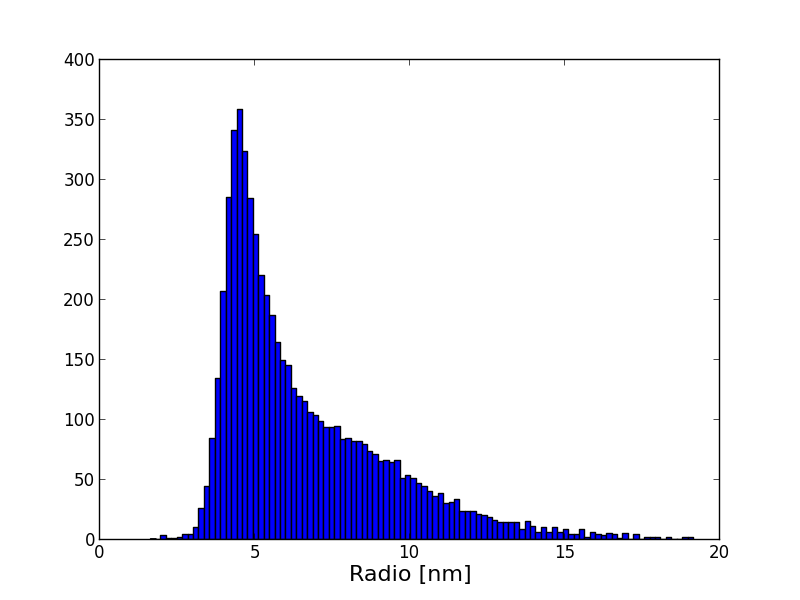
\includegraphics[width=1\linewidth]{hist-radios-5e-6-50-64-160KVm}
	\captionof{figure}{\color{Green} Radios de poros con $\alpha$ = 50\si{\micro\metre}, 160\kvm y t = 5 \usec}
	\end{center}\vspace{1cm}

\columnbreak

	\begin{center}\vspace{1cm}
	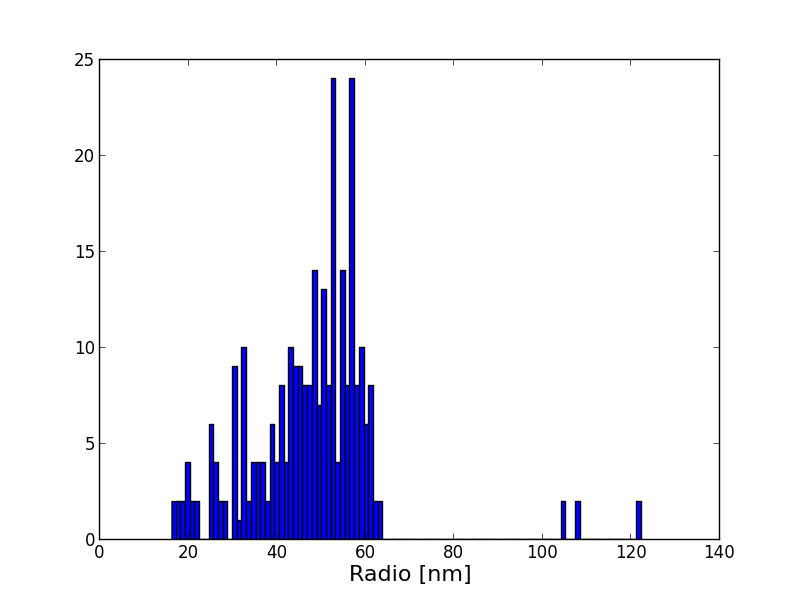
\includegraphics[width=1\linewidth]{hist-radios-5e-3-50-64-160KVm}
	\captionof{figure}{\color{Green} Radios de poros con $\alpha$ = 50\si{\micro\metre} y 160\kvm  y t = 5 \si{\milli\second}}
	\end{center}\vspace{1cm}
\end{multicols}

Sólo los poros grandes (mayores a 1 $\si{\nano\metre}$), son de interés. \\
Si bien se crean muchos poros, éstos se sellan rápidamente con el paso del tiempo: a los 5 $\si{\milli\second}$ del pulso en todos los casos la cantidad de poros es mucho menor en instantes anteriores, aunque los pocos poros grandes que siguen existiendo suelen tener mayor radio que la mayoría de los poros en los instantes anteriores. La corta vida de la mayoría de los poros puede deberse a que la alta densidad de los primeros instantes reduce significativamente la conductancia de la membrana, y por lo tanto el ITV necesario para mantener los poros abiertos.


\section*{Conclusiones}
	\begin{itemize}
		\item Se pueden ingresar las especies, pero se necesitan voltajes muy altos,
			sobre todo para \na y \cl
		\item Los poros generados disminuyen la conductancia de la membrana, 
			disminuyendo el ITV
		\item El voltaje aplicado influye en la velocidad con la que se crean los poros,
			pero no aumenta el ITV, siempre que se alcance un valor mínimo
		\item La mayoría de los poros creados se cierran muy rápidamente; antes de que 
			lleguen las especies, luego no sirven para permeabilizar la membrana
	\end{itemize}


\begin{thebibliography}{9}

\bibitem{puchiar}
	G. Puchiar, T. Kotnik, B. Valič and D. Miklavčič
	\emph{Numerical Determination of Transmembrane Voltage Induced on Irregularly Shaped Cells}
	Annals of Biomedical Engineering
	April 2006, Volume 34, Issue 4, Pages 642-652

\bibitem{krass}
	Wanda Krassowska and Petar D. Filev
	\emph{Modeling Electroporation in a Single Cell}
	Biophysical Journal
	Volume 92, Issue 2, 15 January 2007, Pages 404–417

\bibitem{jianbo}
	Jianbo Lia, Wenchang Tanb, Miao Yua, Hao Lina
	\emph{The effect of extracellular conductivity on electroporation-mediated molecular delivery}
	Biochimica et Biophysica Acta 
	1828 (2013) 461–470

\end{thebibliography}

\end{multicols}
\end{document}